\chapter{Sequence diagrams}

\section{Dataprocessing and -storage}
\begin{figure}[!ht]
	\begin{center}
		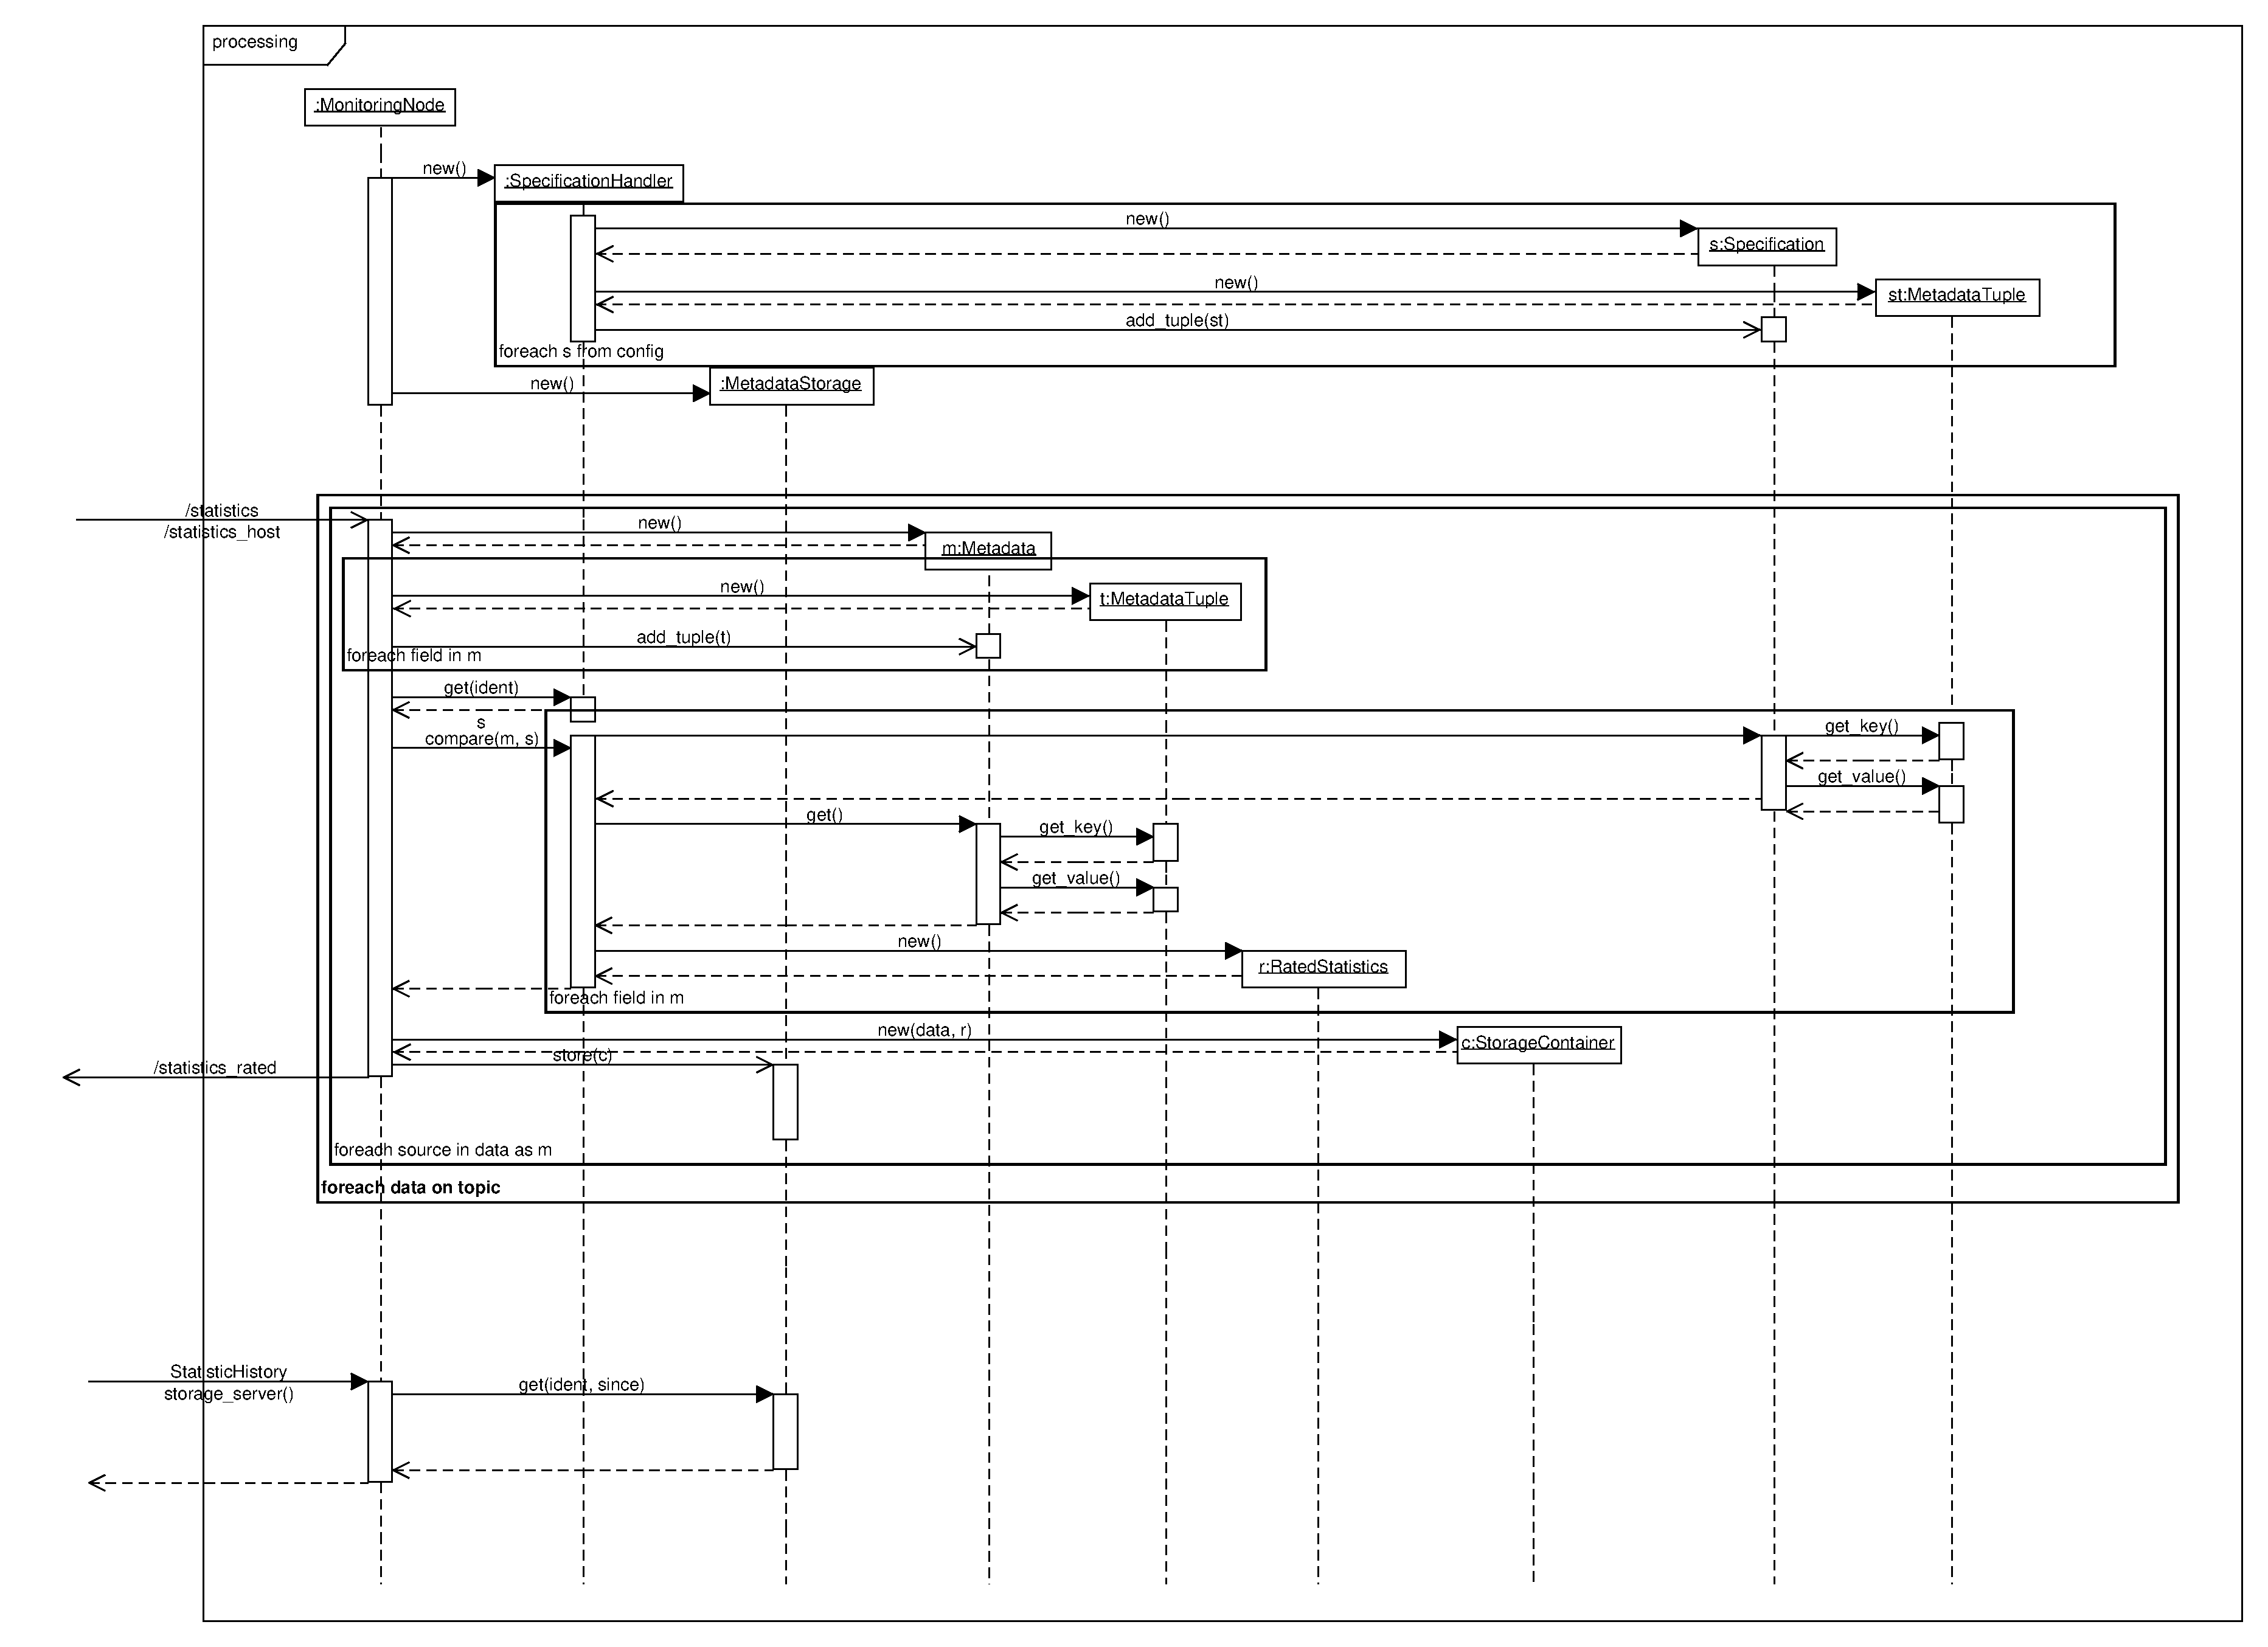
\includegraphics[width=1.0\linewidth]{./diagram_pictures/processing_seq.pdf}
		\caption{Three sequences appearing in the data-processing part of the project.}
	\end{center}
\end{figure}

\subsection*{Setup}
During the first activity of the MonitoringNode, it sets up a SpecificationHandler, which then loads all specifications from config files and stores them in MetadataTuple objects bundled in Specification objects.\\
It then sets up the MetadataStorage.

\subsection*{Receiving data}
The second activity of the MonitoringNode is triggered on receiving data on either the /statistics or /statistics\_host topic. The incoming data is translated into Metadata objects containing of several MetadataTuples describing every measurement featured in the received data.\\
Now the MonitoringNode looks up a Specification from SpecificationHandler concerning the connection/node/host it just received data about.\\
On success it compares the created Metadata object with the found Specification object MetadataTuple-wise for each field featured in the Metadata/Specification object.\\
Erroneous results will be marked in a new RatedStatistics object. Bundled with the raw input data, a timestamp and an identifier describing the concerned connection/node/host it will be stored in the MetadataStorage object created on setup.

\subsection*{Providing data for the GUI}
Answering a request for all data or a special identifier describing a connection/node/host since a given point of time, the MonitoringNode will return the matching data from the MetadataStorage.
A result of that will contain raw data, rated data, a timestamp and the identifier mentioned above.



\newpage
\section{Countermeasures}
\begin{figure}[!ht]
	\begin{center}
		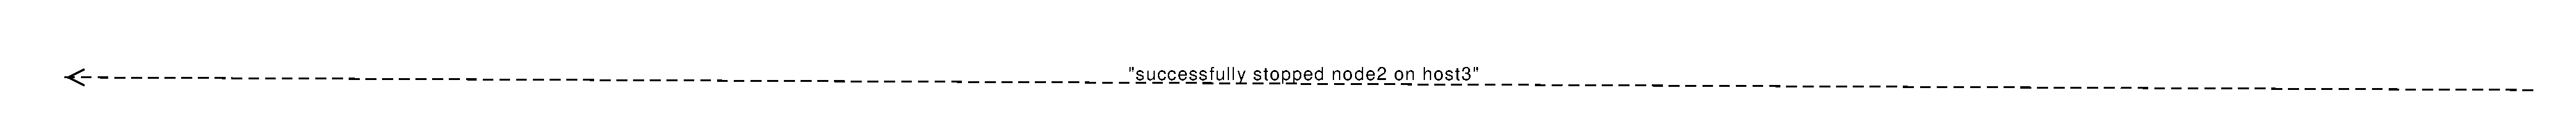
\includegraphics[width=1.0\linewidth]{./diagram_pictures/reactor/reactor_seq.pdf}
		\caption{Initialisation of Constraints and evaluating and executing countermeasures.}
	\end{center}
\end{figure}